\section{Architettura del prodotto}
Dopo un approfondito studio il team ha optato per l'utilizzo del design pattern \textbf{Model View View-Model}, che prevede tre macrosezioni:
	\begin{itemize}
		\item \textbf{Model}: rappresenta i dati contenuti nel sito, ma non i comportamenti o i servizi che manipolano l'informazione. Non è responsabile della renderizzazione;
		\item \textbf{View}: si occupa di rappresentare le informazioni contenute nel sito ed è quello con cui l'utente interagisce; la view in questo design pattern è attiva, al contrario di quello che succede nell'MVC, questo perché contiene comportamenti, eventi e riferimenti a stati del sito, che quindi presuppongo una conoscenza della logica che sta dietro ai dati;
		\item \textbf{Viewmodel}: fornisce i dati dal Model in una forma in cui la View può usufruirne. Si occupa inoltre della logica della vista e di mantenersi costantemente sincronizzato con la View.
	\end{itemize}
Per poter apprezzare questa suddivisione nel pacchetto del team viene riportato qui di seguito il diagramma generale dei package. Si proseguirà successivamente alla descrizione delle implementazioni di ogni sezione in relazione all'architettura della Product Baseline, illustrandone i rispettivi design pattern utilizzati.
\\Per facilitare la comprensione della struttura dei diagrammi delle classi, il team ha deciso di raggruppare tutti i \emph{Containers}, i \emph{Components} e le \emph{actions} nei loro rispettivi packages. Infatti il comportamento di ogni classe di ogni package è modulare:
	\begin{itemize}
		\item Tutti i \emph{Components} importano la classe \emph{React.Component}
		\item Tutti i \emph{Containers} importano il rispettivo \emph{Component}, la rispettiva \emph{Action} e il pacchetto \emph{react-redux}.
		\item Tutte le \emph{actions} importano le \emph{costants} che azionano il \emph{reducer}, il pacchetto \emph{react-router}, lo \emph{store}, il pacchetto \emph{truffle-contract} e la classe \emph{IpfsUtils}
	\end{itemize}
I diagrammi presentati in questo documento illustrano la struttura sinteticamente; la loro versione integrale si può trovare nella cartella Diagrammi.


\begin{figure}[h]
	\centering
	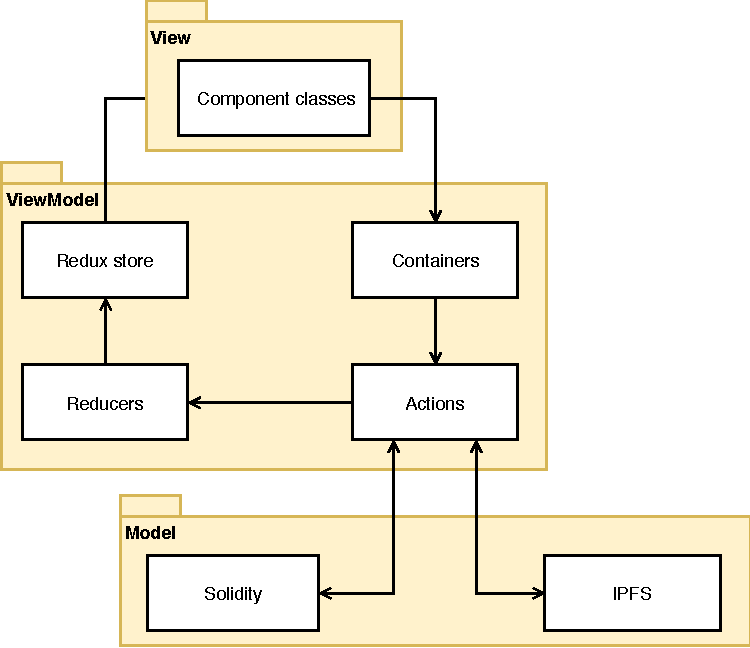
\includegraphics[height=3in]{./Diagrammi/FrameworkPackageGenerale.pdf}
	\caption{Diagramma generale dei package}
	\label{}
\end{figure}

	
	\subsection{View}
		\subsubsection{Design patterns}
		Progettando questa sezione ci si è resi conto che si sarebbero potute generare delle classi \emph{dumb}, ovvero slegate dalla logica del sistema e che si sarebbero dovute occupare solamente della rappresentazione delle informazioni. Per ottenere questo si è ricorso all'utilizzo del seguente design pattern:
			\begin{itemize}
				\item \textbf{Decorator}: sfruttando il macro-package \emph{Container}, che poi si occupa di collegare il componente allo stato di \emph{redux}, si possono decorare tutte le componenti ivi presenti con dei componenti react puri, ai quali vengono passate eventualmente le informazioni e le funzioni a disposizione attraverso un accesso al \emph{this.props}. In questa maniera si ha la completa separazione tra rappresentazione e dati - cosa auspicata dal framework MVVM - e si facilitano modifiche future.
			\end{itemize}
		
		\subsubsection{Diagramma delle classi}
		In Figura~\ref{fig:DiagrammaView} è riportato il diagramma delle classi relativo a questa sezione con evidenziato la posizione del design pattern utilizzato.
	
%	{\textcolor{red}{INSERIRE DIAGRAMMA CON VISTA SU VIEW}}

	
	\subsection{ViewModel}
		\subsubsection{Design patterns}
		Essendo una tra le sezioni più complesse da gestire e quella che poi si sarebbe dovuta occupare della gestione degli stati dell'applicazione, si è deciso di seguire in parte i design pattern offerti dal framework sfruttato e di aggiungerne altri in seguito ad un'analisi più profonda del problema.
		In Figura~\ref{fig:DiagrammaViewModel} si è ricorso all'utilizzo dei seguenti design pattern:
			\begin{itemize}
				\item \textbf{Observer}: implementato già nel framework offerto da Truffle, si occupa di gestire gli stati dell'applicazione sfruttando il framework \emph{react-redux}. Il team lo ha declinato sfruttando la classe \emph{index} come \emph{observer} e la classe \emph{store} come subject. Lo \emph{store} viene aggiornato ogni qual volta si registra un cambiamento nello \emph{state} dell'applicazione, grazie agli strumenti offerti da \emph{redux}; questo aziona l'update dell'\emph{index}, che quindi si occupa di eseguire un render a schermo aggiornando le informazioni cambiate;
				\item \textbf{Fa\c{c}ade}: sfruttato in maniera estensiva, questo pattern ha permesso al team di generare interfacce per semplificare gli import all'interno di classi generali (vedasi, ad esempio, l'import di \emph{index} che deve importare tutte le componenti);
				\item \textbf{Adapter}:\item \textbf{Adapter}: per interagire con i contratti \emph{solidity} \emph{truffle} ha sfruttato alcune componenti come \emph{adapter}: la classe \emph{migrate}, in particolare, si occupa di importare i contratti \emph{solidity}, di farne il \emph{deploy} all'interno della blockchain istanziata e poterli sfruttare come dei più leggibili \emph{json}. Dopodiché la classe \emph{truffle-contract} offre dei metodi per arricchire le istanze dei contratti ottenuti dal deploy con informazioni utili al loro sfruttamento nell'applicazione.
			\end{itemize}
				\begin{figure}[!h]
		\centering
			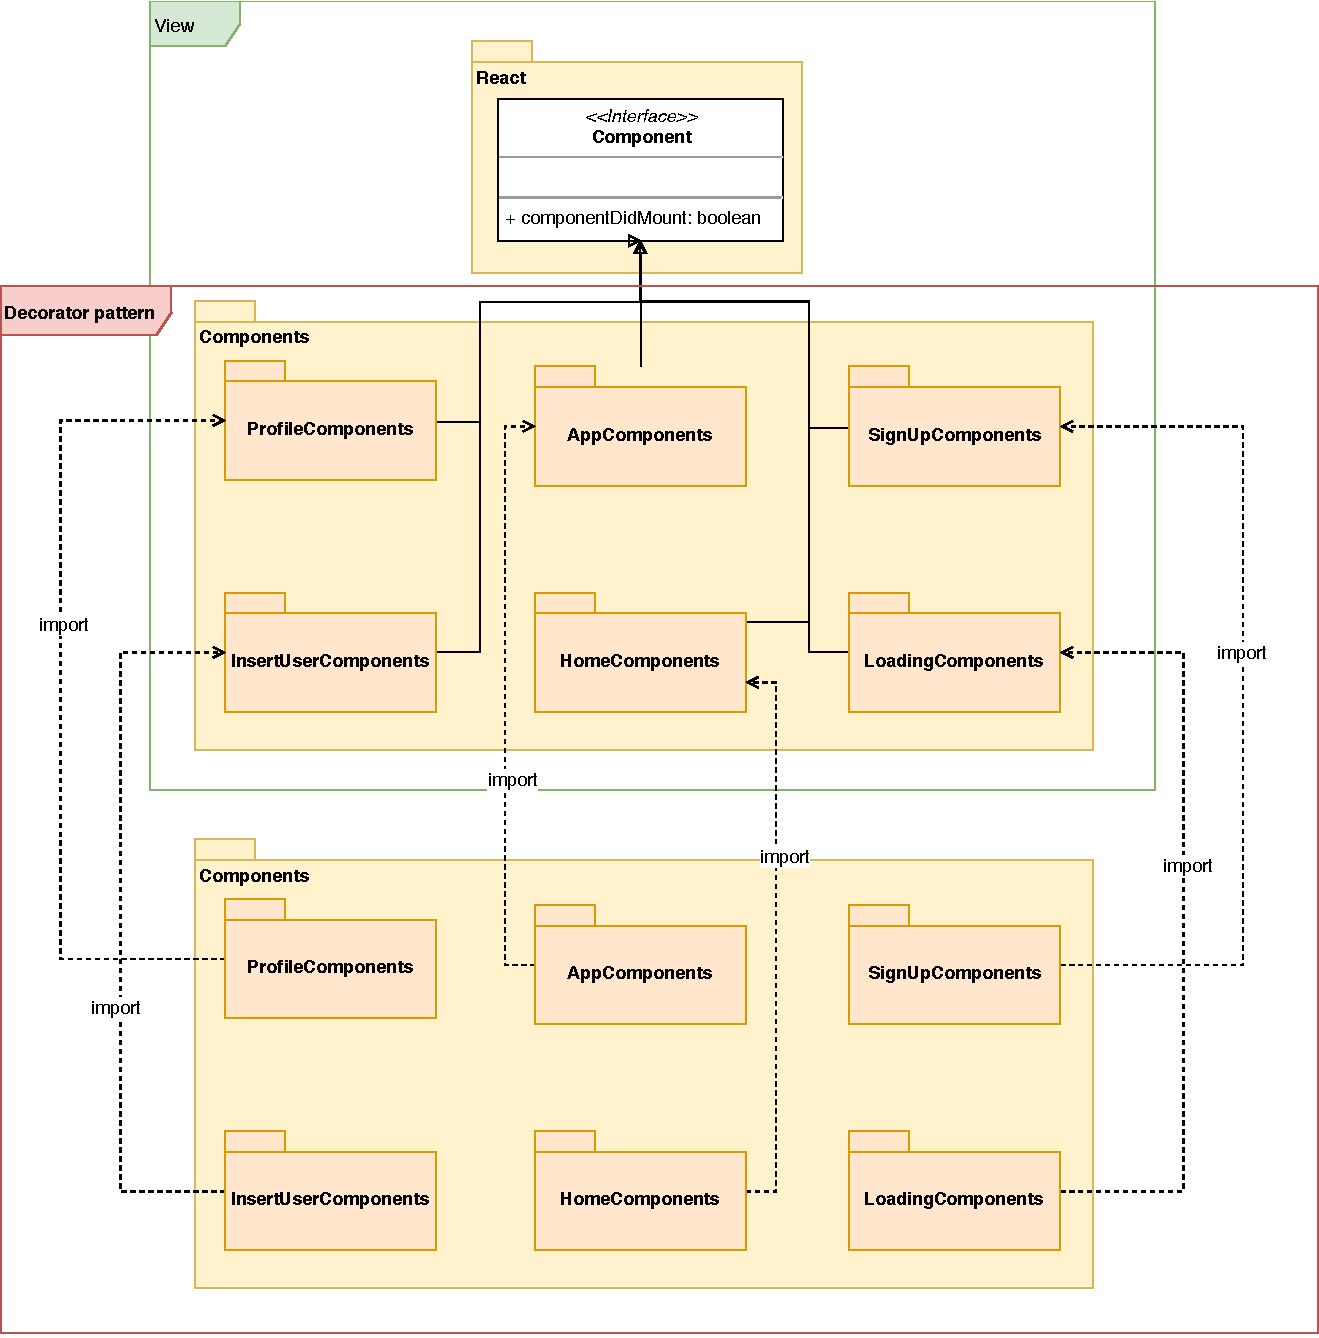
\includegraphics[height=7in]{./Diagrammi/DiagrammaView.pdf}
		\caption{Diagramma delle classi del componente View}
		\label{fig:DiagrammaView}
	\end{figure}
	
		\subsubsection{Diagramma delle classi}
		In seguito è riportato il diagramma delle classi relativo a questa sezione con evidenziato la posizione del design pattern utilizzato.
	
	\clearpage
	\begin{figure}[hp]
		\centering
			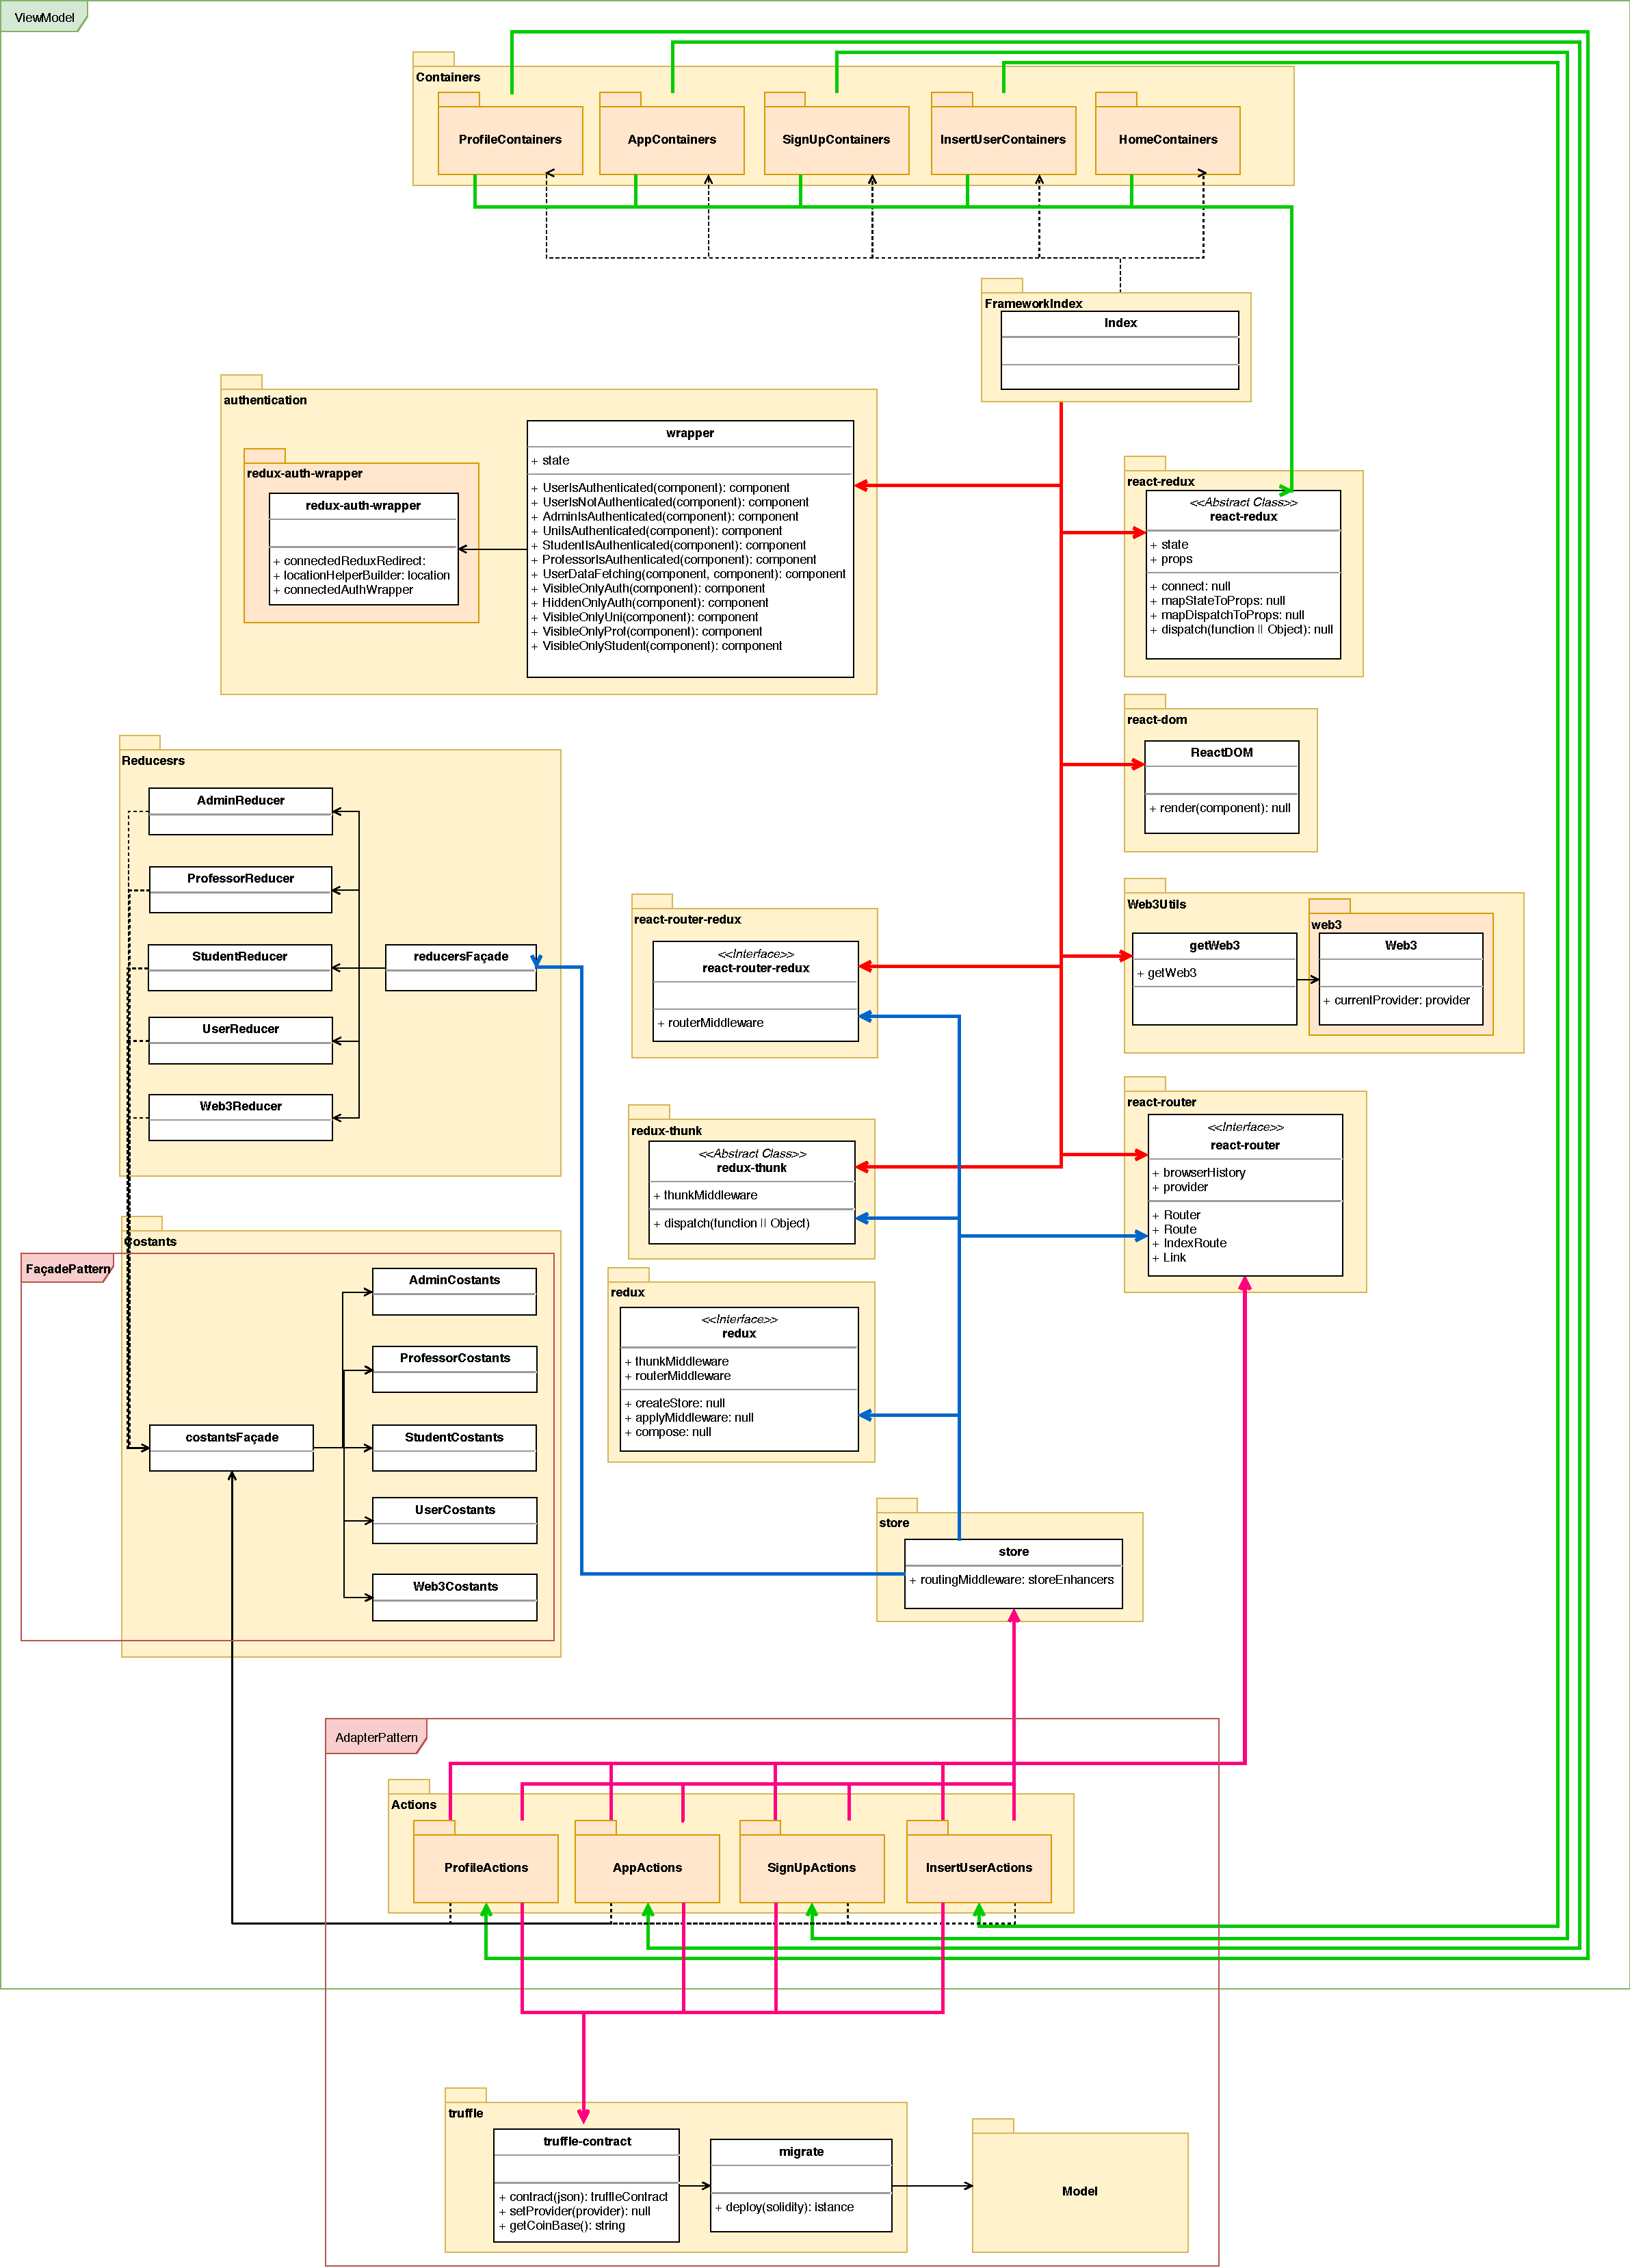
\includegraphics[height=9in]{./Diagrammi/DiagrammaModelView.pdf}
		\caption{Diagramma delle classi del componente ViewModel}
		\label{fig:DiagrammaViewModel}
	\end{figure}
	\clearpage	
	
\subsection{Model}
\subsubsection{Architettura}
		Per quanto riguarda la macrosezione relativa alla componente Model, composta dai contracts salvati su blockchain ed IPFS, si sono effettuate le seguenti scelte progettuali:
		\begin{itemize}
			\item \textbf{Modularità}: dividendo la parte logica e la struttura dei dati, in caso di aggiornamento della parte logica e quindi di un nuovo deploy dei contracts interessati, si ottiene la persistenza dei dati e un minor costo per il nuovo deploy. Infatti, se i dati e la logica fossero salvati nello stesso contracts, ad un nuovo deploy, i dati non sarebbero più consistenti, essendo contenuti in un altro contratto;
			\item \textbf{Istanze di contracts}: ogni contracts ha un'unica istanza: se i contracts contengono oggetti con molteplicità, essi saranno strutturati in una struct e si salveranno in un mapping con una key che li identifica ed una value che punta all'istanza della struct interessata. Si salvano, inoltre, per ogni mapping, un array contenente le key dei mapping. Questo perchè in Solidity (il linguaggio utilizzato per programmare i contracts), non è possibile in alcun modo recuperare quali key sono già salvate nel mapping e quindi si utilizzano gli array collegati per iterare sui dati;
			\item \textbf{Denormalizzazione}: come per altri database di tipo NoSQL e contrariamente ai database relazionali, si deve mantenere un compromesso fra ridondanza dei dati e costo del salvataggio maggiore. Infatti, per ottenere delle query più semplici e veloci, è necessario mantenere la ridondanza dei campi dati utilizzati più spesso. Questo si traduce in una maggior complessità per la modifica e l'eliminazione dei dati, ma si ottengono vantaggi significativi in caso di iterazioni sui dati non dovendo effettuare chiamate a contracts quando una transazione lo richiede e quindi richiedendo un costo minore;
			\item \textbf{IPFS}: il costo del salvataggio dei dati su blockchain Ethereum è molto elevato. Per questo motivo, alcuni dati sono salvati off-chain su un altro sistema distribuito, ovvero IPFS. La scelta di salvare un dato su blockchain Ethereum o su IPFS segue quindi queste regole:
			\begin{enumerate}
				\item I dati utilizzati come identificativo per le query sono salvati su blockchain
				per evitare la latenza dovuta alla comunicazione fra backend-frontend-IPFS;
				\item I dati soggetti a problemi di concorrenza sono salvati su blockchain: in questo modo
				non serve porsi il problema dell'accesso concorrenziale per la modifica del dato da parte
				di molteplici utenti in contemporanea;
				\item Tutti i dati considerati "accessori" possono essere salvati su IPFS.
			\end{enumerate}
		\end{itemize}
		\subsubsection{Diagramma delle classi}
		In seguito è riportato il diagramma delle classi relativo a questa sezione con evidenziato la posizione del design pattern utilizzato.
	
\clearpage	
	\begin{figure}[h]
		\centering
			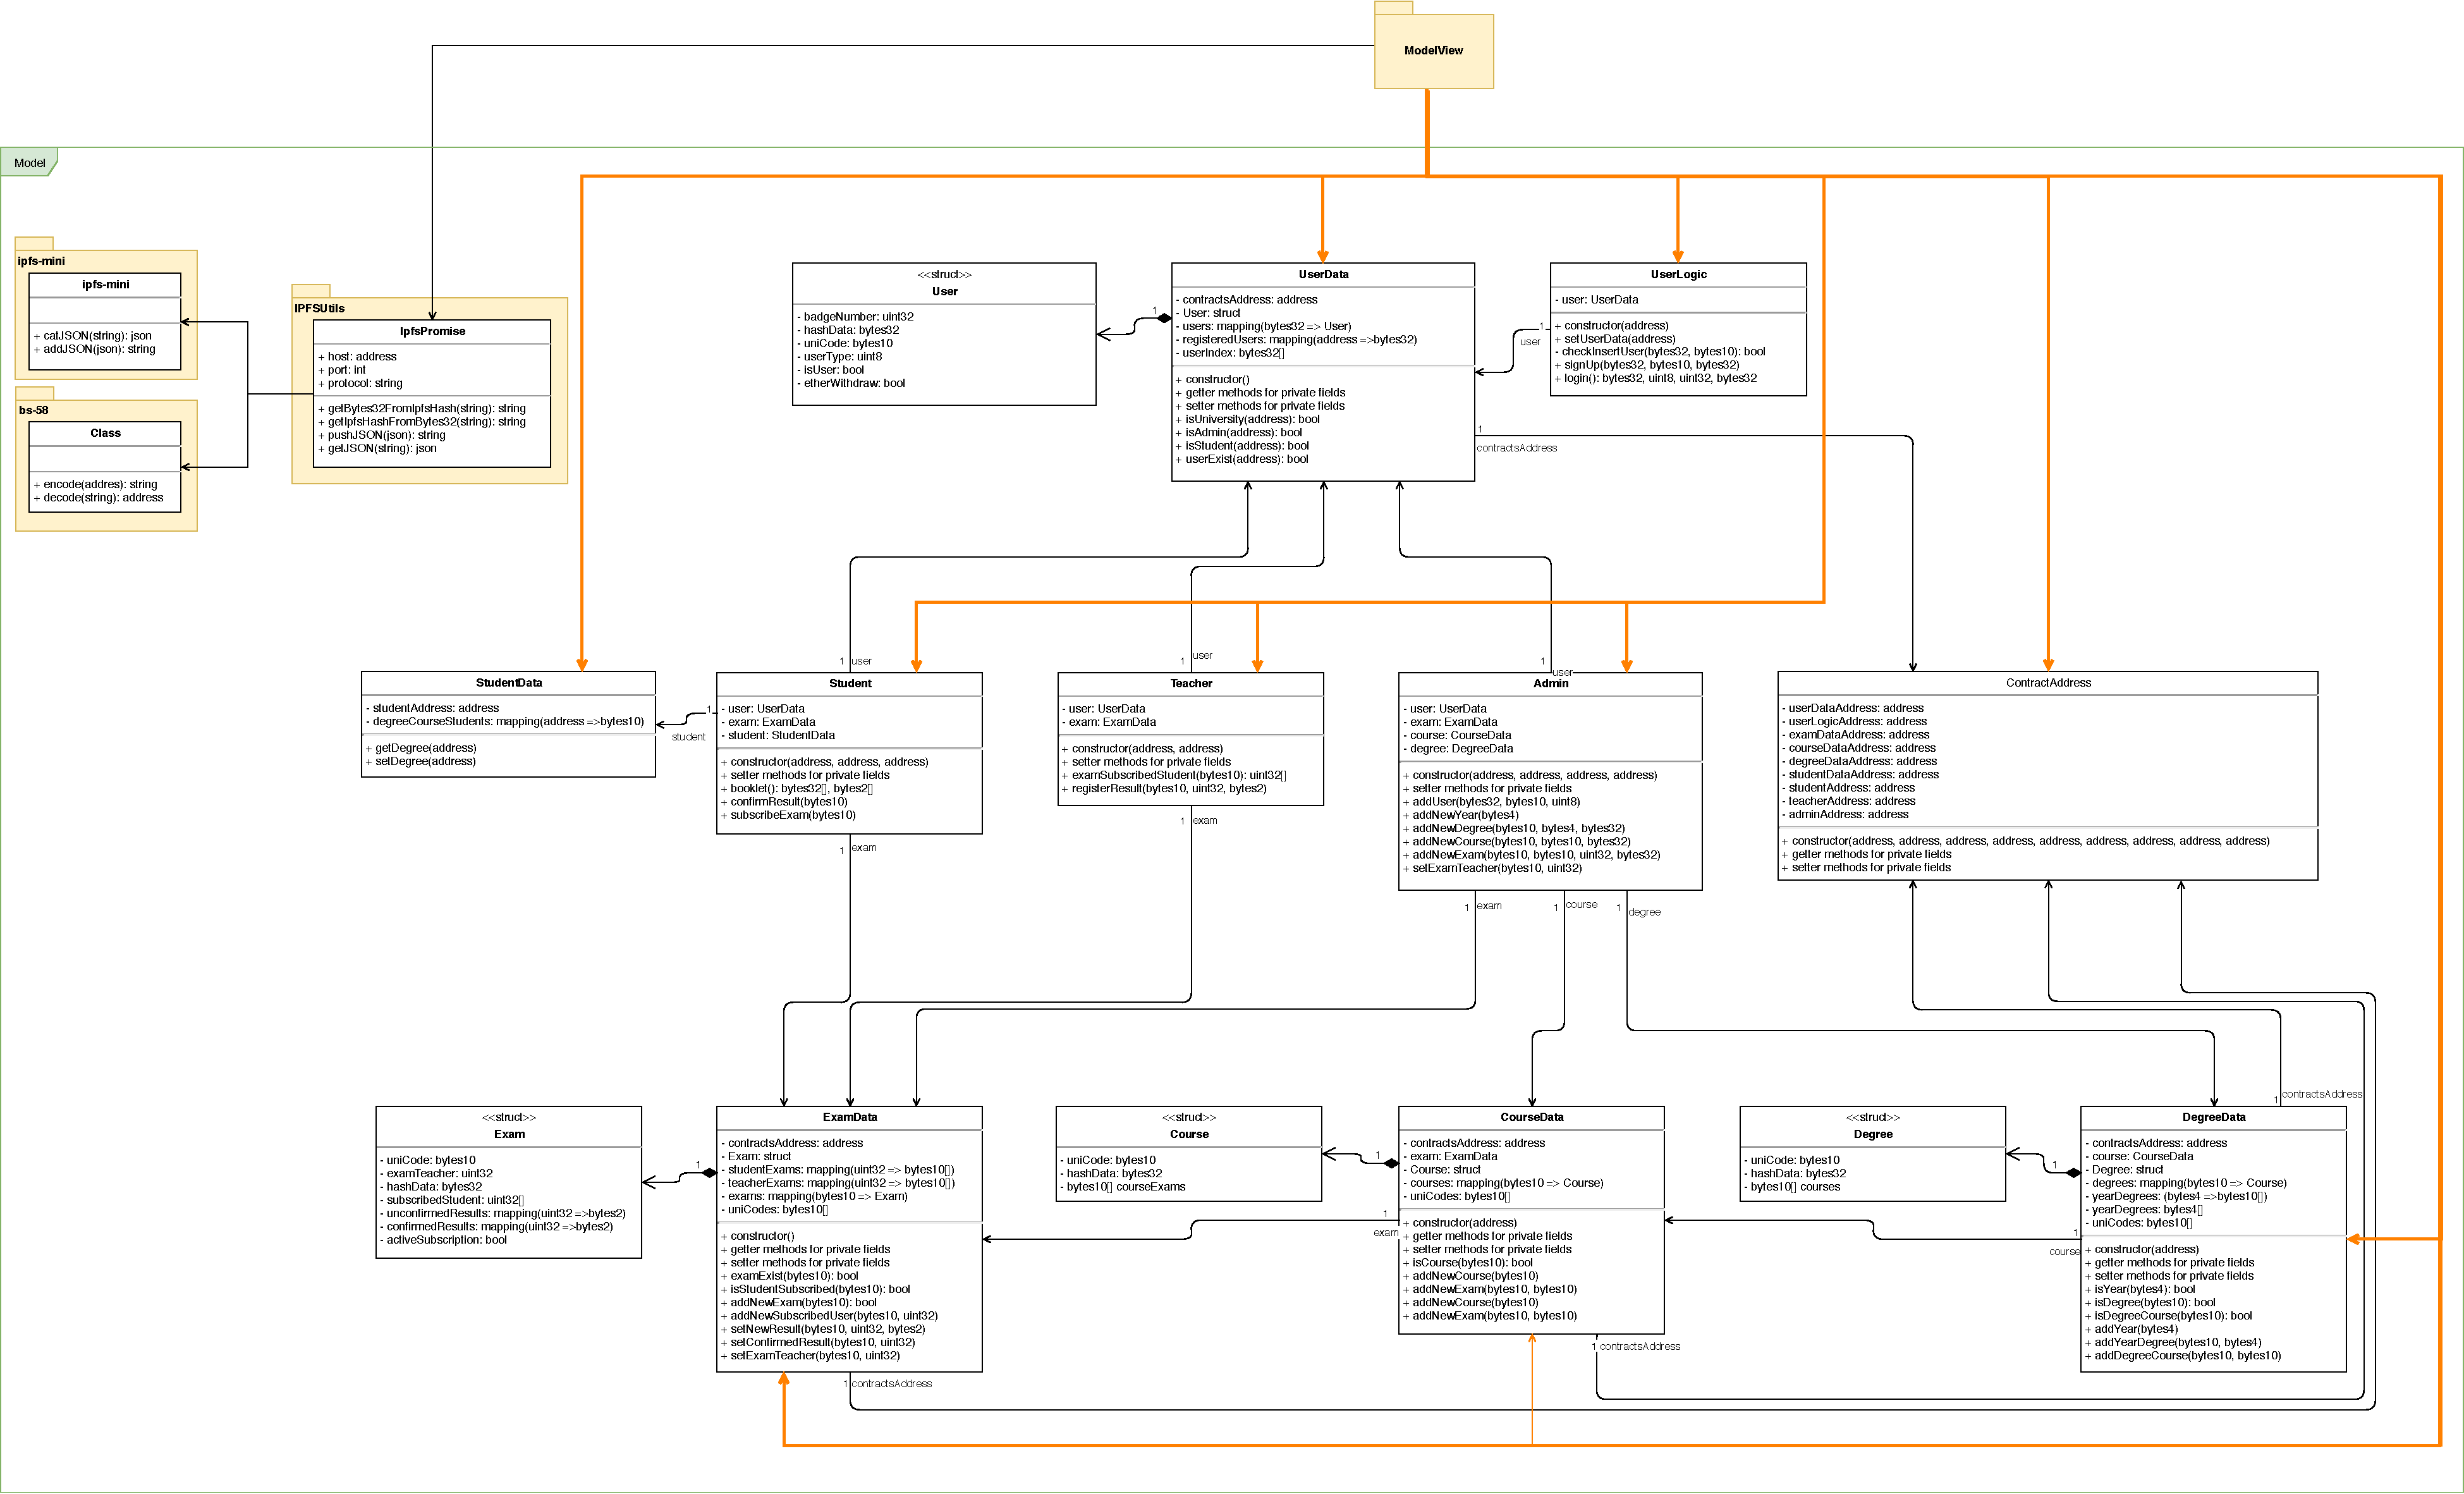
\includegraphics[angle=90, origin=c, height=7in]{./Diagrammi/DiagrammaModel.pdf}
		\caption{Diagramma delle classi del componente Model}
		\label{}
	\end{figure}
		\clearpage
	
	\subsection{Diagrammi di sequenza}
	Come per i diagrammi delle classi, sono stati redatti i seguenti diagrammi di sequenza, disponibili e meglio visualizzabili nella cartella Diagrammi;
	
		\subsubsection{Login}
		Il diagramma di sequenza riportato qui di seguito raffigura il processo di login, durante il quale l'utente che vuole accedere può essere autenticato dal sistema.
		
		\begin{figure}[h]
			\centering
				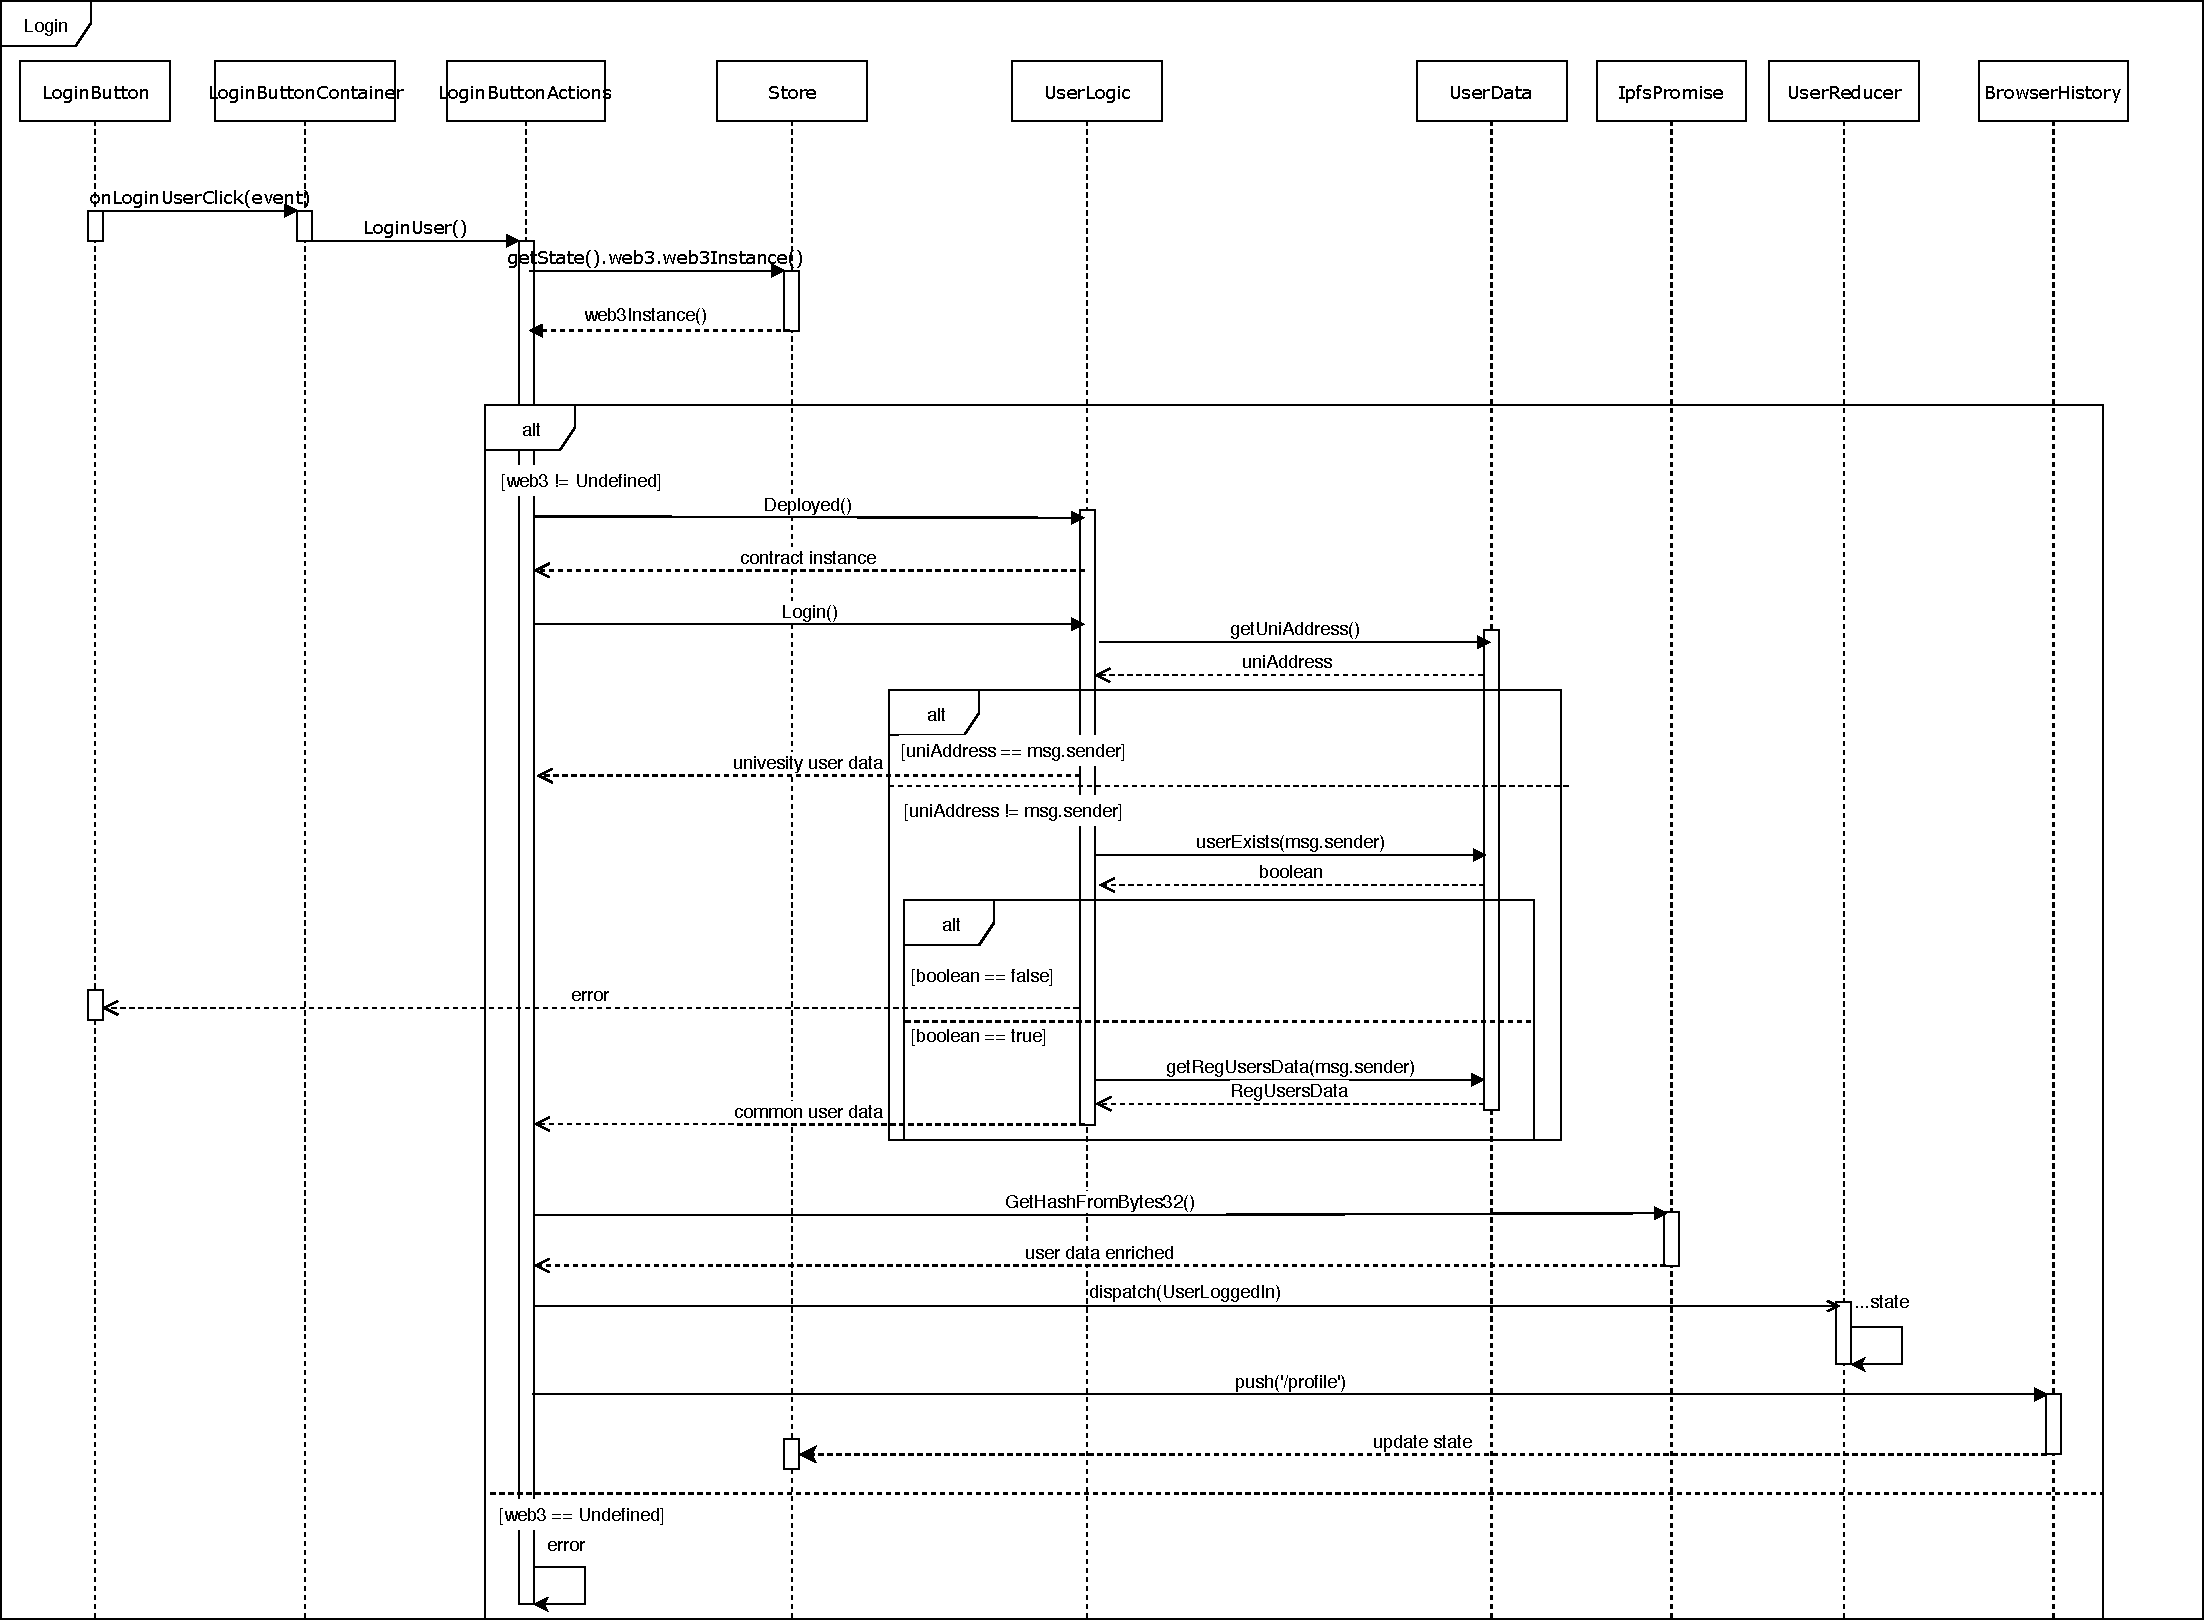
\includegraphics[height=5in]{./Diagrammi/DiagrammaSequenzaLogin2.pdf}
			\caption{Diagramma di sequenza del processo di login}
			\label{}
		\end{figure}
		
		\subsubsection{Inserimento di un utente}
		Il diagramma di sequenza in Figura~\ref{fig:SeqInserimentoUtente} rappresenta l'azione di inserimento di un utente nel sistema.
		\begin{figure}[h]
			\centering
				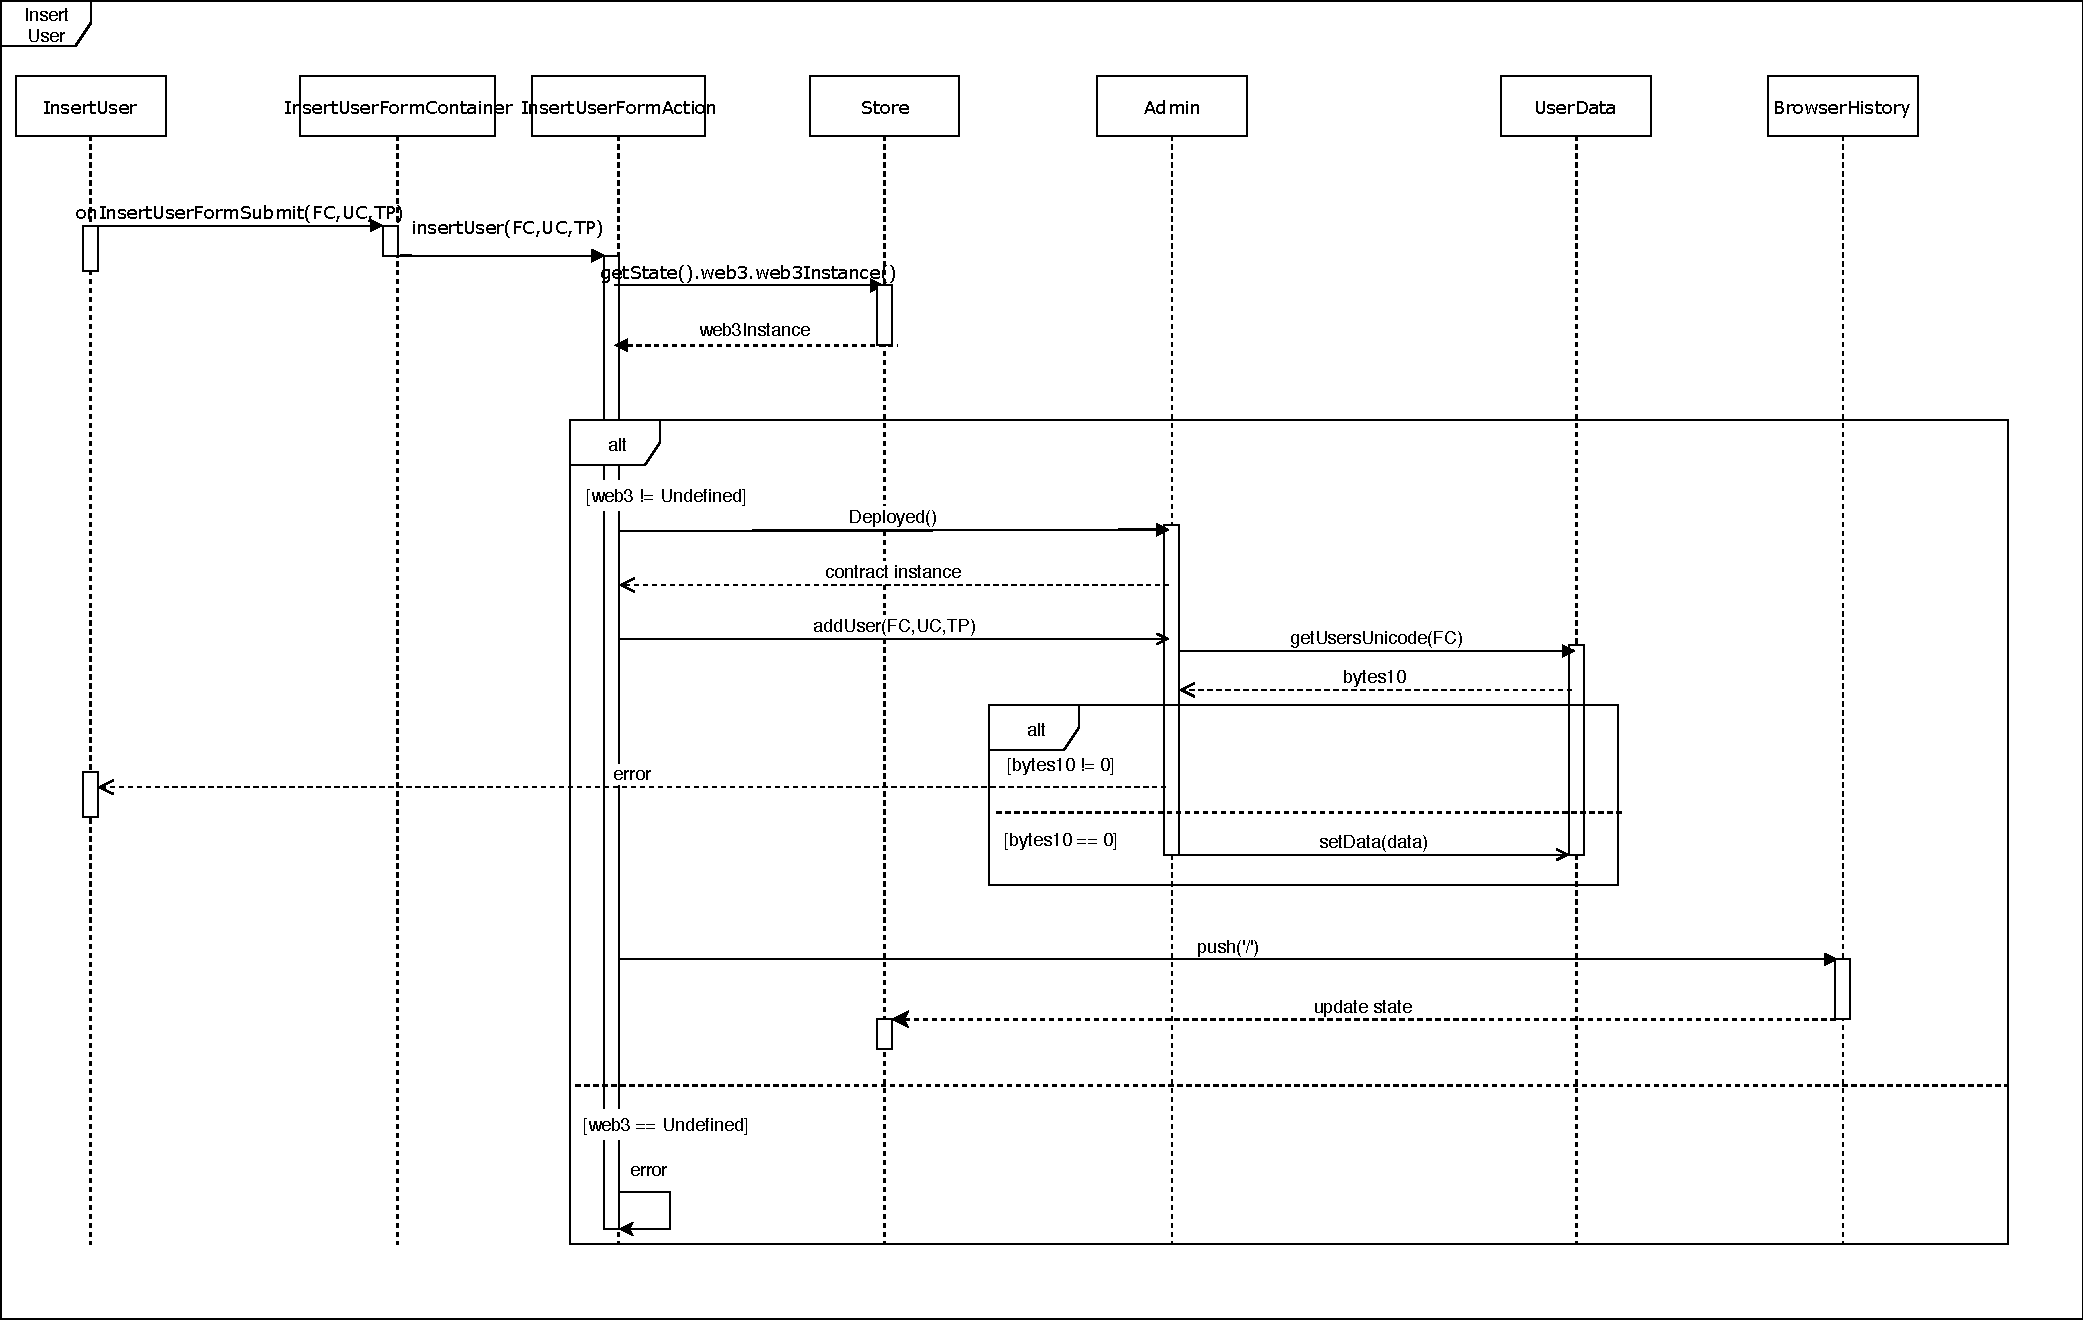
\includegraphics[height=4.5in]{./Diagrammi/DiagrammaSequenzaInsertUser.pdf}
			\caption{Diagramma di sequenza del processo di inserimento di un utente}
			\label{fig:SeqInserimentoUtente}
		\end{figure}
		
		\subsubsection{Inserimento di un anno accademico}
		Il diagramma di sequenza riportato in Figura~\ref{fig:SeqInsertYear} raffigura il processo di inserimento di un nuovo anno accademico nel sistema.
		
		\begin{figure}[h]
			\centering
				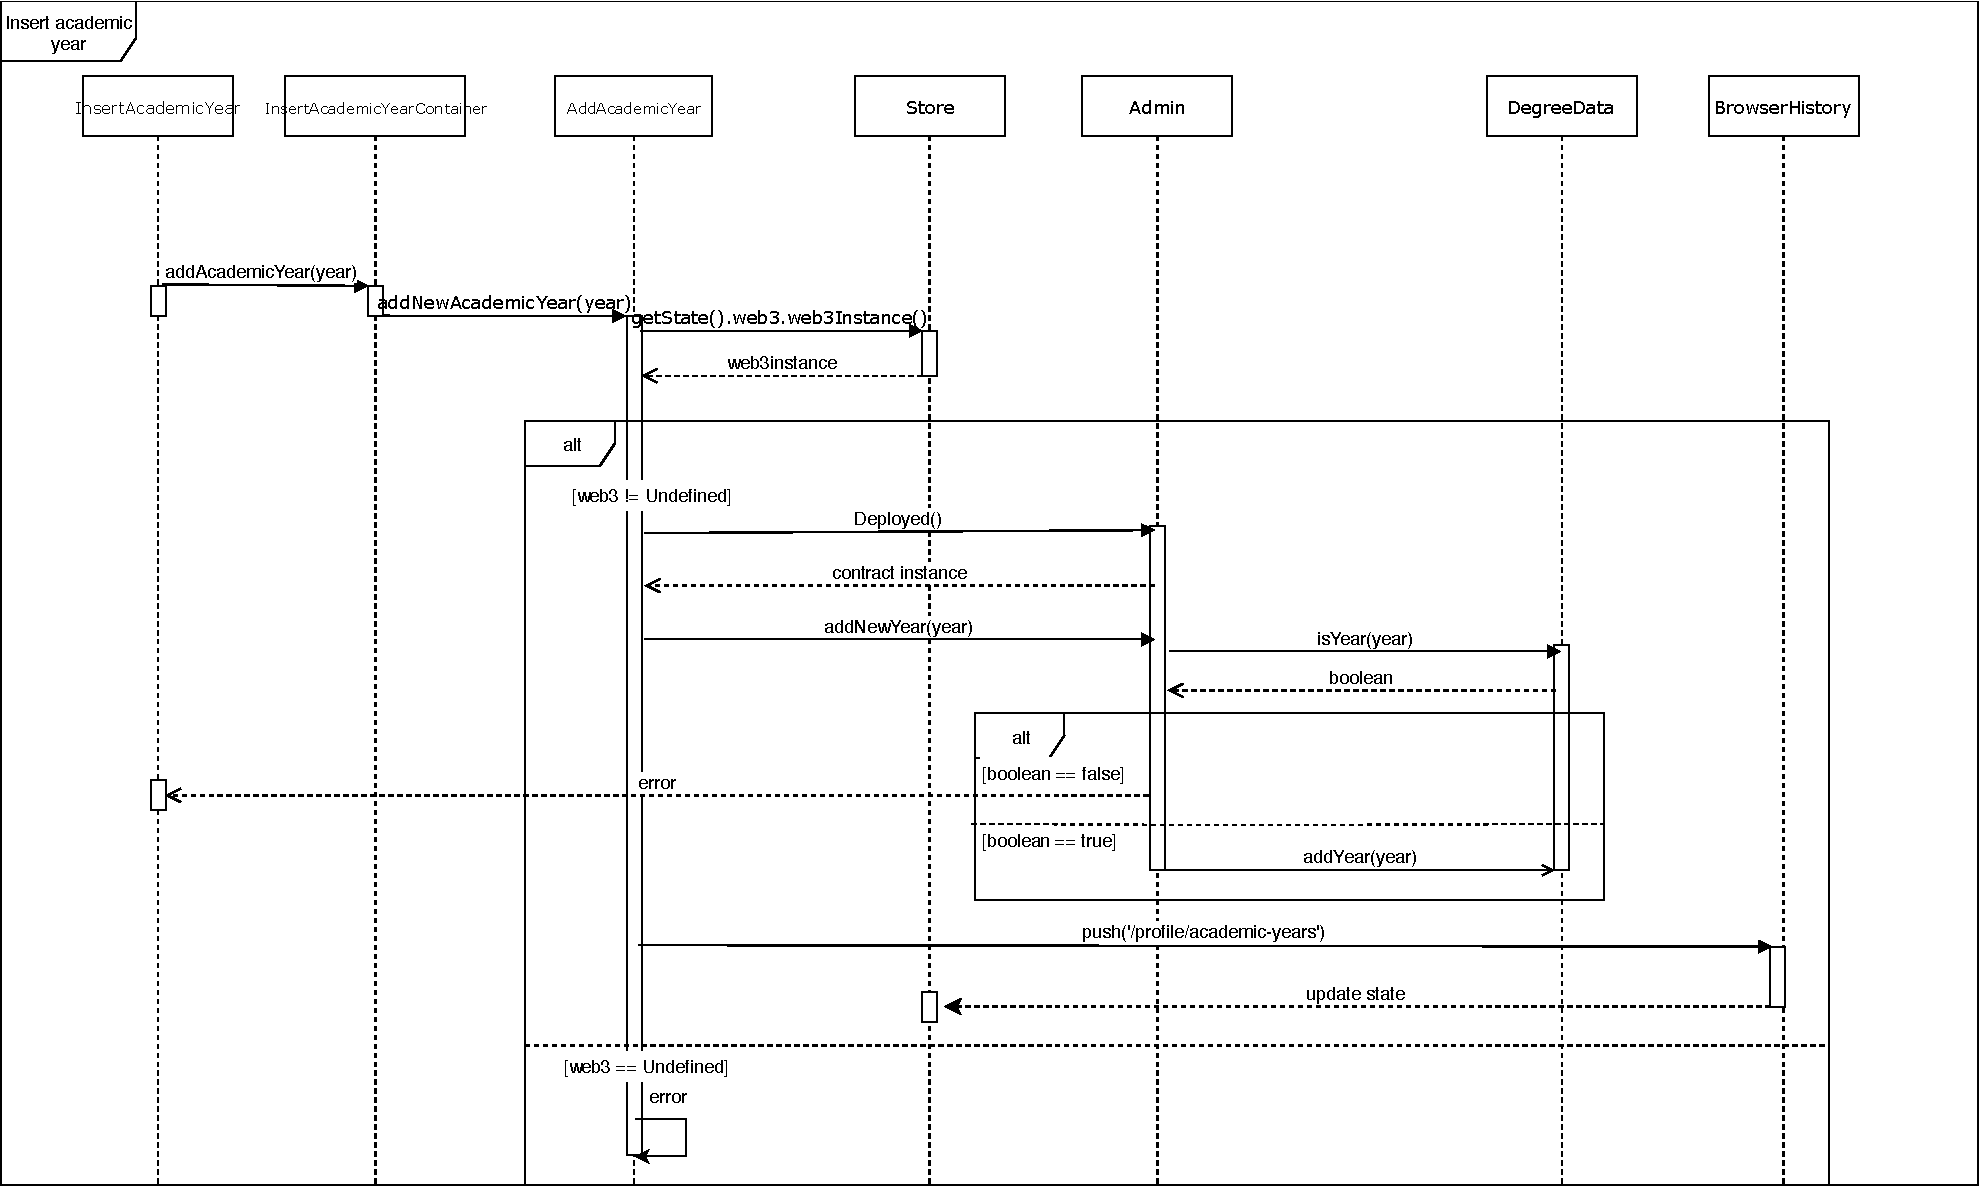
\includegraphics[height=4in]{./Diagrammi/DiagrammaSequenzaInsertAcademicYear.pdf}
			\caption{Diagramma di sequenza del processo di inserimento di un anno accademico}
			\label{fig:SeqInsertYear}
		\end{figure}
		\clearpage
		
	
	
	
	
	